% IEEEtran initializes legacy Times metrics before fontspec enables Unicode text.
\def\encodingdefault{OT1}
\documentclass[journal]{IEEEtran}
\usepackage{iftex}
\ifPDFTeX
  \usepackage[T1]{fontenc}
  \usepackage{microtype}
\else
  \usepackage{fontspec}
  \setmainfont{texgyretermes}[
    Extension=.otf,
    UprightFont=*-regular,
    BoldFont=*-bold,
    ItalicFont=*-italic,
    BoldItalicFont=*-bolditalic]
  \usepackage[expansion=false]{microtype}
\fi
\usepackage{amsmath}
\usepackage{array}
\usepackage{booktabs}
\usepackage{graphicx}
\usepackage{placeins}
\usepackage{xurl}
\newcommand{\pending}[2]{\par\smallskip\noindent\textbf{Pending [#1].} #2\par\smallskip}

\title{Cross-Map Representation and Generalization of Defensive Openings in Counter-Strike 2}
\author{Working draft: author details pending}
\begin{document}
\maketitle
\noindent\textit{Working draft. Source verification, permissions and declarations await author review.}

\begin{abstract}
Defensive openings in Counter-Strike 2 develop as players take positions, move and allocate resources. Comparing these openings across maps requires a shared representation of what is observed, together with a test of what transfers. We extend single-map opening analysis to six maps using geography, player state, relative height and sampled motion with explicit missing-data masks. Four graph/nongraph and static/recurrent encoders learn to reconstruct an entire opening window, after which patterns and retrieval are fitted using training matches. Development uses 465 windows from nine series. Frozen models are evaluated on another 246 windows from 12 series, with the target map excluded from training. The recurrent graph model has a geometric mean reconstruction-loss ratio of 1.016 against its nongraph recurrent control, with a model-based 95 percent interval of 0.996 to 1.036. Joint context makes development clusters repeatable, but equipment dominates their separation. The study provides a controlled cross-map analysis and identifies a central interpretation risk: stable clusters can mainly reflect resources. Independent tactical retrieval relevance and coaching efficacy remain unconfirmed. % [claim:C180] [evidence:E110,E124,E126,E131]
\end{abstract}
\begin{IEEEkeywords}
Counter-Strike 2, defensive deployments, representation learning, cross-map generalization, graph models.
\end{IEEEkeywords}

\section{Introduction}
At the start of a Counter-Strike 2 (CS2) round, five counter-terrorist (CT) players establish a defensive formation. Their positions, spacing, movement and available resources provide observations of how the opening develops. TAGNet uses a sequence of such observations to discover defensive patterns on Dust2~\cite{tagnet2026}. Extending this analysis to other maps raises a practical question: how can openings be compared when their place names and spatial layouts differ? % [claim:C222] [evidence:E205]

The original study explicitly leaves multi-map transfer, vertically structured maps and a jointly trained temporal module as future directions. It uses twenty Dust2 place categories and planar player distances; a shared representation must address the loss of map-specific place detail, differences in height and the evolution of the same players through time. These are the starting points of the present study, rather than an assumption that a successful single-map partition already defines universal defensive categories. % [claim:C223] [evidence:E205,E101,E103]

We approach the problem through observable deployment information. A location identifies where a player is; its tactical meaning also depends on the other players, movement, resources and information that may not be recorded. We therefore describe openings using a common set of geographic categories, player states, relative geometry and sampled motion. The goal is to retain comparable observations while allowing their interpretation to depend on the particular opening.

Our contribution is a controlled extension from single-map pattern analysis to cross-map opening representations. First, we define a common observation space with explicit survival and missing-data masks. Second, we train graph and nongraph encoders with the same window reconstruction target, and compare static averaging with learned temporal aggregation. Third, we fit patterns and retrieval on training matches and apply the fixed procedure to new series whose map is absent from encoder training. Separate context controls test what changes when equipment, score and utility are given explicit weight. The contribution lies in this representation, training and evaluation design; its components do not constitute a new graph or recurrent architecture. % [claim:C183] [evidence:E101,E107,E124,E130,E131]

The experiments form a connected test of that extension. We first check which observations survive the common description, then compare how the four encoders retain them, and finally examine transfer and the meaning of the resulting groups. The central findings concern learned temporal aggregation and resource-sensitive clustering: the new-series comparison does not establish a graph advantage, while highly repeatable context clusters can be dominated by equipment. These findings guide how opening representations should be evaluated before they are used as tactical reference.

\begin{figure*}[t]
\centering
\begin{tabular}{c@{$\;\longrightarrow\;$}c@{$\;\longrightarrow\;$}c@{$\;\longrightarrow\;$}c}
\fbox{\parbox[c][1.5cm][c]{.19\textwidth}{\centering\small CT opening window\\Five snapshots\\Players, pairs, masks}} &
\fbox{\parbox[c][1.5cm][c]{.19\textwidth}{\centering\small Shared encoding\\Graph or MLP\\Static or recurrent}} &
\fbox{\parbox[c][1.5cm][c]{.19\textwidth}{\centering\small Learn on training data\\Reconstruct the window\\64-dimensional vector}} &
\fbox{\parbox[c][1.5cm][c]{.19\textwidth}{\centering\small Apply fixed procedure\\Source-fitted clusters\\Retrieve source windows}}
\end{tabular}
\caption{Study workflow. The reconstruction objective trains the encoder, including the recurrent path when present. Clusters, distance scales and retrieval libraries are fitted using training matches. New series are evaluated without updating these components. Equipment, score and utility can be added to clustering and retrieval as separate context controls.}
\label{fig:workflow}
\end{figure*}

\section{Related Work}
\subsection{From single-map patterns to transferable representations}
TAGNet is the reference for the original snapshot-reconstruction and defensive-pattern task~\cite{tagnet2026}. We distinguish its feature vocabulary, context branch, aggregation implementation, and clustering analysis from the present common-input and learned-temporal variants.

TAGNet learns snapshot features and then combines them with context to form a round representation. In the released author manuscript, reconstruction reads each snapshot before aggregation, so the GRU and context projection retain their seeded initialization; reported pattern clustering uses embeddings from all reported rounds. Our decoder instead reconstructs the full window from its final representation, training the temporal path, and our centroids are fitted only on training embeddings. This changes the learning task and transfer protocol. Absolute losses therefore cannot be compared directly with TAGNet, and our graph/nongraph result does not refute its single-map result. % [claim:C206] [evidence:E205,E107,E111]

\subsection{Team and spatial representations}
Deep Sets develops a framework for permutation-invariant set functions~\cite{NIPS2017_f22e4747}. Janossy pooling constructs invariance through averaging an order-sensitive function over reorderings~\cite{murphy2019janossy}. Our existing five-player non-graph control applies this symmetrization principle to jointly permuted nodes and edge endpoints. It serves as a comparator and is not presented as a new pooling algorithm.

X-Ego learns team-level video representations and evaluates teammate/opponent location prediction; its reported dataset uses Mirage and a round-based partition~\cite{wang2025xego}. Our offline CT-window task uses structured team observations, rather than enforcing individual first-person visibility, and addresses a different endpoint. % [claim:C201] [evidence:E201,E103]

Durst et al. learn movement control for CS:GO Retakes on Dust2~\cite{durst2024move}. Human-like movement generation is distinct from retrieving comparable observed openings. Their map-specific training design does not supply a zero-shot multi-map result for the present task. % [claim:C202] [evidence:E202,E109]

Xenopoulos et al. derive directed navigation-graph distances and contextual action values~\cite{xenopoulos2020valuing}. Their spatial example distinguishes asymmetric traversal from Euclidean proximity. Our current geometry is therefore described as an observation, not a validated navigation or tactical-role relation. % [claim:C203] [evidence:E203,E101]

\subsection{Generalization protocols and cluster interpretation}
Gulrajani and Lopez-Paz emphasize the role of architecture, experimental conditions and model selection in domain-generalization comparisons~\cite{gulrajani2020domain}. WILDS organizes evaluation around explicit real-world distribution shifts~\cite{koh2021wilds}. We accordingly distinguish unseen series, training-held maps and chronological transfer; newly acquired data alone do not establish a future-only test. % [claim:C207] [evidence:E206,E207]

Von Luxburg's overview distinguishes stability mechanisms under idealized and actual K-means optimization~\cite{luxburg2010stability}. Its assumptions matter when interpreting agreement across fits. Our stability diagnostics characterize a chosen observation space; an interpretation as defensive duties requires additional evidence. % [claim:C208] [evidence:E208]

Graded cumulative-gain evaluation accommodates nonbinary relevance judgments~\cite{jarvelin2002gain}. Buckley and Voorhees examine the sensitivity of evaluation to incomplete judgments~\cite{buckley2004incomplete}. We therefore describe the old rated-subset replay as a conditional diagnostic, and do not infer full-library relevance from it. The exponential gain and missing-value rules are specified separately in our protocol. % [claim:C209] [evidence:E210,E211]

Together, these studies motivate evaluating three distinct properties: retention of the chosen observations, transfer to held-out matches and maps, and usefulness as tactical reference. Our experiments address the first two computationally; the existing judged material supplies only a limited pilot for the third.

\section{Opening Windows and Study Data}
\subsection{Deployment window and available observations}
A CT opening is represented by observations at 10, 12, 15, 18, and 20 seconds after freeze time. Current inputs contain five consistent player identities, positions, named places, health, equipment, and validity information. Identity is used for alignment and provenance; team identity and future outcomes are not common encoder inputs.

The current input contract requires all five supplied observation times and at least one live CT at every time. Consequently, the evaluated task is conditional on this window availability and does not cover arbitrary early-ending rounds or frames in which all CT players have already been eliminated. % [claim:C125] [evidence:E107]

\subsection{Development cohort}
The existing development cohort contains nine series, 22 Demos, six maps, and 465 eligible CT windows. Seventy-four windows contain casualties. Survival and valid-pair masks remain explicit. All nine series have already been inspected and cannot be relabeled as an untouched final cohort.

\begin{table}[t]
\caption{Recorded cohorts. A casualty window contains at least one CT observed dead at a supplied time; it is not a count of deaths or independent players.}
\label{tab:data}
\centering
\begin{tabular}{lrr}
\toprule
Item & Development & New series\\
\midrule
Series & 9 & 12\\ % [claim:C210] [evidence:E144]
Demos & 22 & 12\\ % [claim:C211] [evidence:E144]
Maps & 6 & 6\\ % [claim:C212] [evidence:E144]
Eligible CT windows & 465 & 246\\ % [claim:C213] [evidence:E144]
Windows with casualties & 74 & 41\\ % [claim:C214] [evidence:E144]
\bottomrule
\end{tabular}
\end{table}

\subsection{New series and pilot judgments}
The external technical cohort is fixed at twelve new series, with one selected map per series, two series per map and four series from each of three events. Acquisition, content-duplicate checks, native clocks, one format-based prelisted replacement and one early-ending exclusion are recorded with checksums. For each target map, the evaluated encoder was trained with that map and all series containing it excluded. Repeated teams and the mixed May/October acquisition do not establish unseen-team or future-only generalization. % [claim:C184] [evidence:E129,E130]

Native parsing yields 246 eligible CT windows from 247 completed rounds; one window ends before the final supplied time. The prelisted same-event Mirage alternate replaces a primary archive containing split map fragments, before any model output. Newly acquired series include May and October matches, so this is not a chronological future-only split or an entirely researcher-unseen map evaluation. % [claim:C170] [evidence:E130]

Existing participant returns and developer-involved AI silver judgments remain separate pilot sources with incomplete coverage. They do not establish the formal independent tactical endpoint. Previously distributed unanswered items are not automatically reopened.

\section{Method}
\subsection{A shared description of an opening}
Figure~\ref{fig:workflow} summarizes the procedure. Each input is a short team history, rather than a tactical label: five observations of the same five players are converted into a shared description, compressed into one vector, and compared with training openings. Context can subsequently change which source openings are considered close. All scaling, cluster fitting and candidate selection are learned or fixed before evaluating new series. % [claim:C224] [evidence:E101,E107,E111,E121,E129]

The shared geographic vocabulary is BombsiteA, BombsiteB, CTSpawn, TSpawn and other. Together with health, equipment and survival, it provides eight node channels. This deliberately coarse vocabulary gives the maps a common interface; it cannot retain every local callout or make positions with the same category tactically equivalent. Relative height, ground state and motion supply observations that these categories and planar spacing omit.

The shared input has 15 channels per player: the eight base fields, five height/ground descriptors and two sampled-motion quantities. Each player pair has three channels for relative geometry. Navigation-mesh projection fields are excluded. % [claim:C101] [evidence:E101,E103]
No tactical-role labels are supplied to the encoder or its loss. A category such as BombsiteA identifies geography on the current map; it does not label the player's responsibility. Interpretation therefore concerns the particular recorded opening and its available context. % [claim:C102] [evidence:E101,E103]
Dead players retain their alignment across times, but their invalid node and pair observations are zero-filled and masked. Feature masks also distinguish an unknown physical measurement from a valid zero; ground state has an explicit unknown indicator. Raw place names are retained for tracing a representation back to its observations. % [claim:C103] [evidence:E101,E103,E107]

Throw counts, facing/visibility and explicit round-level score/economy fields are outside the common encoder input. Recorded score and utility can instead enter the separate context comparison described below; unavailable context is never assumed known. % [claim:C108] [evidence:E101,E103,E121]

A constructed diagnostic illustrates why motion is added. It compares a stationary team with a team translating together while coarse place membership, resources and relative formation are held fixed. The 13 node channels without motion and three pair channels remain identical, whereas the two motion quantities distinguish the constructed windows. Endpoint displacement still cannot recover an intervening out-and-back path or horizontal direction. This is an information-retention check, not a measured tactical effect. % [claim:C109] [evidence:E101,E103]

For each player, the two appended quantities are horizontal displacement magnitude and signed vertical displacement between adjacent supplied observations, divided by elapsed seconds and a fixed scale of 250 game units per second. Identities align endpoints even when player order changes. Both endpoints must be alive; the first observation and invalid intervals are zero-filled and masked, whereas observed stationarity remains a valid zero. Only the current and preceding observations are used. The scale is not a speed bound, and values are not clipped. These quantities retain neither the intervening path nor horizontal movement direction. % [claim:C110] [evidence:E101,E103]

Native height and ground-state observations enter with their validity masks. Navigation-mesh candidates, patch-matching flags and ray diagnostics remain separate audits. The model therefore makes no claim of verified walkability, connectivity or visibility from its geometric inputs. % [claim:C185] [evidence:E101,E103,E129]

\subsection{Encoding the formation and its evolution}
Both encoder families receive the observed feature values, their validity masks and survival indicators. The graph model projects each player to 64 dimensions and applies two attention layers. Each layer combines query--key similarity with a learned linear bias from the three pair channels; dead players are excluded as attention keys. The nongraph control instead jointly flattens the players and pair matrix, uses a 128-to-64 hidden mapping, and averages over all consistent player reorderings. Thus both families can use pair information, while organizing interactions differently. % [claim:C225] [evidence:E107]

A player's input slot should not change the representation, but a player's trajectory should remain consistent. We therefore follow each graph-encoded player through the five times before pooling players. The nongraph model similarly follows each joint reordering through the full window. Recurrent conditions read these sequences in order; static conditions average their encoded time points. Both receive the same sampled-motion fields. This comparison tests the learned temporal representation under shared observations.

For each window, let $X_t$, $A_t$, and $M_t$ denote node observations, pair information, and masks. Let $H_{t,u}$ be the encoded state of a player track or a consistently ordered whole-window permutation view. Temporal encoding precedes invariant pooling:
\begin{equation}
 z=\frac{1}{U}\sum_{u=1}^{U}\mathrm{GRU}_{\phi}(H_{1,u},\ldots,H_{5,u})_5.
\end{equation}
Here $U=5$ for the graph model's player tracks and $U=120$ for the nongraph model's joint node/edge reorderings. The same identity alignment is used throughout a window; player identity itself is not an encoder feature. % [claim:C120] [evidence:E107]

\subsection{Learning by reconstructing the whole window}
Reconstruction provides a training signal without requiring tactical labels: the compressed vector must recover the chosen observations of the entire opening. A consistent relabeling of the five players should produce the same loss. Matching players independently at every time would instead discard trajectory identity, so one assignment is used across the complete window and all pair endpoints.

The four core conditions and two input ablations (Supplementary Appendix~A) share a 64-to-128-to-525 decoder: five times by five anonymous player slots by 15 node channels, plus five times by ten unordered player pairs by three pair channels. The reconstruction loss averages seven groups: survival binary cross-entropy, live-player coarse-region cross-entropy, resource MSE, relative-height MSE, ground-state cross-entropy, known-motion MSE and valid-pair MSE. Each group averages its valid entries, with an empty group contributing zero. A single jointly permuted player assignment across all times and pair endpoints minimizes the window loss over 120 assignments. Survival, region and ground outputs are logits; continuous outputs remain unconstrained regressions. % [claim:C121] [evidence:E107]
\begin{equation}
 \mathcal{L}_i=\min_{\pi\in S_5}\frac{1}{7}
 \sum_{g=1}^{7}\ell_g(\widehat{Y}_i,\pi\!\cdot\!Y_i;\pi\!\cdot\!M_i).
\end{equation}
Here $Y_i$ contains all node and pair targets for window $i$, $\widehat{Y}_i$ is the decoder output, $M_i$ is the validity mask, and $\ell_g$ is one group loss. The set $S_5$ contains the 120 player reorderings. The same $\pi$ acts at every supplied time and on both pair endpoints.

\subsection{Adding observed match context}
The separate context vector contains five log-transformed CT equipment totals, the two pre-round public scores and thirty log-transformed CT utility counts: six types at each of the five supplied times. Counts start at freeze end and stop at the current query time. A missing required group makes that context policy unsupported, while policies using available groups remain evaluable. These are recorded observations, not active utility areas or inferred intentions. % [claim:C215] [evidence:E118,E121,E140,E147]

The node representation already includes individual equipment. Consequently, adding equipment context repeats an aggregate view of information partly present in the encoder; the branches are not disjoint information sources. Our controls vary the retrieval or clustering contribution of explicit context. They do not enforce resource-invariant embeddings, orthogonality or statistical independence, and the term deployment representation does not assert that equipment information has been removed. % [claim:C216] [evidence:E103,E107,E147]

\section{Evaluation Design}
\subsection{Training and transfer conditions}
We use two development conditions. In series exclusion (G3), an entire match series is absent from training and validation. In map-and-series exclusion (G4), the target map and every series containing that map are excluded. G4 therefore tests whether a representation learned on the remaining maps can describe the held-out map. The new-series evaluation reuses the corresponding G4 checkpoints and source libraries; no new series enters those libraries. This procedure was frozen locally before acquiring the new archives, rather than externally preregistered.

All six conditions were trained from scratch under the fixed development recipe: AdamW with learning rate $10^{-3}$ and weight decay $10^{-4}$, batch size 16, 100 epochs, gradient clipping at 5, and seeds 0, 1 and 42. The earliest epoch minimizing source-validation reconstruction was selected. Nine series-exclusion folds and six map-plus-series-exclusion folds yielded 270 selected checkpoints; pilots were excluded. The graph and MLP models share input observations, 64-dimensional bottlenecks and the decoder, but their parameter counts are not exactly matched. % [claim:C122] [evidence:E109,E110]

\subsection{What the evaluation measures}
Reconstruction loss measures recovery of the recorded observations, with lower values better. Clustering asks whether similar vectors form repeatable groups. Cross-seed adjusted Rand index (ARI) measures agreement between two group assignments; a value of one means identical partitions on the evaluated windows. Coverage is the fraction admitted by a source-fitted support and radius rule. These are different properties: a repeatable group need not be a useful tactical category, and high coverage does not establish accurate interpretation.

For retrieval, a query is ranked against actual training windows. We inspect the returned observations and vary the influence of recorded context. Newly generated rankings lack independent relevance judgments; the complete old judged-pool replay, including its discounted-gain definition and all scores, is retained in Supplementary Appendix~B-C.

The development pattern-analysis implementation uses scikit-learn~\cite{pedregosa2011sklearn}. Candidate cluster counts are two through six, selected solely by source-training silhouette; the query embeddings do not select or refit centroids. Numeric cluster IDs are retained without tactical names. A source-radius and minimum-support rule records rejected queries as a diagnostic, with cross-seed agreement reported only where both assignments are accepted and vary across at least two clusters. The separate source-series bootstrap fixes the neural encoder and selected cluster count. % [claim:C204] [evidence:E111,E112,E204]

Transfer reuses the saved source centroids, cluster support and 95th-percentile source radius with minimum support five. It does not refit on new windows. We report both coverage and cross-seed adjusted Rand index on common accepted windows, requiring multiple clusters in each assignment. Eligibility can differ between methods, so their ARI summaries are conditional diagnostics. Source-series bootstrap variability fixes the encoder and source-selected cluster count. % [claim:C186] [evidence:E111,E114,E134,E137]

\subsubsection{How context changes comparison}
To determine whether adding context changes what a group represents, we mix a representation distance with distances between observed equipment, score and throw counts. Each component is scaled using training matches so that a high-dimensional group does not automatically dominate because it contains more coordinates.

For a source vector group of dimension $d$, let $a$ be its mean squared Euclidean distance over distinct source pairs. Centering by the source mean and dividing by $\sqrt{a}$ gives unit mean source-pair distance; numerically constant groups use denominator $\sqrt{d}$. Context groups are scaled separately and receive equal weight within the selected group set $G$. Thus the ranking distance is % [claim:C219] [evidence:E121,E147]
\begin{equation}
 D_\lambda(q,s)=(1-\lambda)d_z(q,s)
 +\frac{\lambda}{|G|}\sum_{g\in G}
 \|\widetilde{c}_{g,q}-\widetilde{c}_{g,s}\|_2^2.
\end{equation}
The same source-only scaling applies to embedding distances. Statistics first use their recorded source-fitted feature standardization; complete observation matching normalizes its permutation-minimized distance by the mean distinct-source-pair distance. Joint clustering concatenates the correspondingly square-root-weighted vectors. Context-only drops the representation term. All means and scales are source-fitted, including when query availability changes. % [claim:C220] [evidence:E121,E123,E147]

\subsection{How new-series uncertainty is estimated}
The new-series technical comparison uses series as its analysis unit. Frames, rounds and seeds are aggregated within series rather than counted as additional independent series. Existing development prediction intervals are conditional descriptive series-resampling summaries; they do not remove shared-team or overlapping-training dependencies.

For map $m$ and its two series $j$, let $r_{mj}$ be the log ratio of the series-averaged Graph+GRU and MLP+GRU losses. We estimate the equal-map mean and its residual standard error as % [claim:C218] [evidence:E131,E132]
\begin{equation}
 \widehat{\mu}=\frac{1}{6}\sum_{m=1}^{6}\overline{r}_m,
 \qquad
 \widehat{\mathrm{SE}}=\sqrt{\frac{1}{72}\sum_{m=1}^{6}s_m^2}.
\end{equation}
Here $\overline{r}_m$ and $s_m^2$ are the mean and sample variance of the two series log ratios for map $m$. The common-variance interval uses six residual degrees of freedom. The prespecified unequal-variance sensitivity changes the critical value using Welch--Satterthwaite degrees of freedom, retaining the same point estimate and standard error. These model-based intervals assume independent normal series residuals; they are not design-based guarantees.
The primary quantity is the graph/recurrent loss divided by the nongraph/recurrent loss on new series, summarized on the log scale with equal map weight. A ratio below one favors the graph condition; a ratio above one favors the nongraph control. The pooled interval and its unequal-variance sensitivity do not remove shared-team/event dependence. Other conditions are descriptive, and no model, context weight or sample size is selected from the new-series results. % [claim:C187] [evidence:E129,E131,E132]

\section{Results}
\subsection{What the common representation retains}
The first question is whether a shared input retains the observations needed to compare openings. The five-category vocabulary permits common dimensions, but leaves substantial local position detail unresolved.

The shared five-category vocabulary maps 50.57--81.01\% of live observations to other across the six maps. This is our cross-map common vocabulary, not TAGNet's twenty-place Dust2 vocabulary. The large other category motivates retaining geometry and motion alongside coarse geography; reducing its size alone would not establish tactical correctness. Detailed per-map counts are in Supplementary Appendix~B. % [claim:C105] [evidence:E101,E104,E205]

\subsection{What graph structure and learned time aggregation add}
We next ask which encoder best retains the same observations. The four core conditions separate the organization of player interactions from learned time aggregation, while keeping the target fixed.

The complete development matrix covers the same 465 windows under each exclusion regime, rather than 930 independent windows. We average seed-specific losses within each window, then within each series, and finally weight the nine series equally. Table~\ref{tab:mainrec} reports the seven-group reconstruction objective; it is not a tactical accuracy score. % [claim:C123] [evidence:E110]

\begin{table}[t]
\caption{Core architecture comparison for development reconstruction. Lower is better. Every condition reconstructs the same shared target; three seeds are averaged before equal-series aggregation.}
\label{tab:mainrec}
\centering\small
\begin{tabular}{lrr}
\toprule
Condition & G3 & G4\\
\midrule
MLP, static & 0.104151 & 0.130487 \\ % [claim:C130] [evidence:E110]
MLP + GRU & 0.091641 & 0.123633 \\ % [claim:C131] [evidence:E110]
Graph, static & 0.101017 & 0.130968 \\ % [claim:C132] [evidence:E110]
Graph + GRU & 0.092370 & 0.125391 \\ % [claim:C133] [evidence:E110]
\bottomrule
\end{tabular}
\end{table}

Temporal graph and MLP conditions reduced the objective against their static counterparts by 8.56\%/4.26\% and 12.01\%/5.25\% in G3/G4, respectively. Graph + GRU nevertheless had 0.79\%/1.42\% higher loss than full-input MLP + GRU. The corresponding descriptive paired reduction intervals were [-2.54, 0.69]\% and [-3.36, 0.25]\%; a stable graph advantage is not established. These conditional series-resampling summaries do not remove shared-team or overlapping-fold dependence. % [claim:C124] [evidence:E110]

The two input-reduction conditions, the paired motion analysis and the complete per-series reconstruction plot are reported in Supplementary Appendix~A. Supporting component and telemetry audits are in Supplementary Appendix~B.

\subsection{What the discovered groups represent}
A representation can reconstruct observations yet produce groups with a different organizing principle. We therefore examine stability first, then ask whether the stable groups primarily reflect deployment information or the added resource context.

Source-only cluster selection and assignment were completed for all 270 encoder fits. For example, the full graph-temporal condition selected two clusters in 24 of its 27 G3 fits, rather than recovering a predetermined six-pattern taxonomy. Table~\ref{tab:stability} reports descriptive agreement and diagnostic assignment coverage; numeric cluster IDs are local to each fit and do not name duties. % [claim:C127] [evidence:E114]

\begin{table*}[t]
\caption{Core-architecture pattern diagnostics; input reductions are in Supplementary Appendix~A. ARI is averaged over fold/seed pairs on their common accepted queries; different K and method-specific eligible subsets limit direct comparisons. G3 has 27 computed pairs for each condition. G4 pair counts show missing comparisons. G4 coverage pools 1,395 query-seed assignments per condition, not independent samples.}
\label{tab:stability}
\centering\small
\begin{tabular}{lrrrr}
\toprule
Condition & G3 ARI & G4 ARI & G4 computed pairs & G4 coverage (\%)\\
\midrule
MLP, static & 0.684 & 0.582 & 18/18 & 83.7 \\ % [claim:C140] [evidence:E114]
MLP + GRU & 0.353 & 0.520 & 18/18 & 86.0 \\ % [claim:C141] [evidence:E114]
Graph, static & 0.578 & 0.534 & 16/18 & 85.8 \\ % [claim:C142] [evidence:E114]
Graph + GRU & 0.502 & 0.406 & 18/18 & 93.0 \\ % [claim:C143] [evidence:E114]
\bottomrule
\end{tabular}
\end{table*}

With context, full graph-temporal seed ARI was 1.000 in G3 and 0.995 in G4; full MLP-temporal ARI was 0.983 and 0.988. G4 diagnostic assignment coverage was 90.2\% and 91.3\%, respectively. All these neural context fits selected two source clusters. Different accepted query subsets still limit comparisons with the state-only table. % [claim:C153] [evidence:E123]

The increase in stability raises a further question: what separates the resulting groups? A post-hoc decomposition of the source-centroid distances provides a concrete answer. For G4 Graph + GRU with context, state coordinates contributed 2.66\% of squared centroid separation, equipment 66.55\%, score 6.34\%, and utility 24.45\%. Its query partition agreed with context-only clustering at mean ARI 0.987 on eligible common assignments. These are properties of the normalized representation, not causal feature importance. Stable resource groups do not establish tactical duties; deployment descriptions and contextual facets remain separate. % [claim:C154] [evidence:E124]

The inspection of retrieved windows is a separate step. Figure~\ref{fig:deployment} shows one fixed query and the actual source candidates returned by two encoders. The raw positions and observed displacement links make the returned evidence inspectable, although they cannot establish why a player moved or whether the opening is a good tactical reference.

An exact-stimulus audit checked the old packet hashes and displayed coordinates, places, health and equipment against the same frozen windows. Restricting candidates to the current source-training library leaves 17 complete numeric pairs across three queries. A sensitivity subset retains existing numeric scores without requiring the original completion flag: 30 usefulness and 29 similarity records across five queries. Original scores, missing values and abstentions remain unchanged. % [claim:C155] [evidence:E125]

The pilot is too small and selectively judged to resolve the relevance of these new returns. The restricted old judged-pool replay and new rankings have different evidential roles. No old grade is transferred to a new query or candidate pair. The new-series ranking outputs remain unjudged, so turnover, source-radius acceptance and pattern agreement do not establish reference quality, tactical responsibilities or coaching value.

\begin{figure*}[t]
\centering
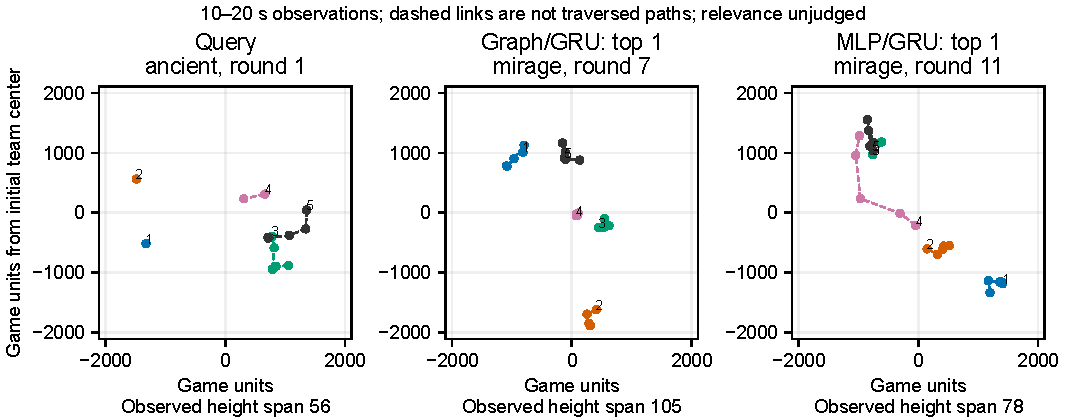
\includegraphics[width=\textwidth]{figures/de_ancient.pdf}
\caption{The fixed first Ancient G4 query and the top cross-map candidates from full-input graph/GRU and MLP/GRU, seed zero. Coordinates are centered at each window's initial live-team center with native axes and a shared scale; colors identify players within each panel only. Dashed links connect observed endpoints, not traversed routes. Walls, opponents and utility are absent, and relevance remains unjudged.}
\label{fig:deployment}
\end{figure*}

\subsection{What survives transfer to new series}

The final test applies the procedure without retraining to new series on maps omitted from the corresponding encoder training. This distinguishes performance on the development folds from transfer of a fixed procedure. Figure~\ref{fig:independent} reports every series rather than only the pooled estimate.

All 108 corresponding source checkpoints were reused without training or test-side selection. For each series, we first average losses across its windows and three seeds, then compute the Graph+GRU to MLP+GRU log ratio. The equal-map estimate is 0.01564 log units, or a geometric loss ratio of 1.01576; the pooled normal-residual 95\% interval is [0.99586, 1.03606] on the ratio scale, with six residual degrees of freedom. This is not the ratio of the two grand arithmetic means. % [claim:C171] [evidence:E129,E131]

The prespecified unequal-variance sensitivity gives a ratio interval of [0.98218, 1.05049], with Welch--Satterthwaite degrees of freedom approximately 2.075. Anubis has the largest observed within-map separation. Two series per map cannot verify normal residuals; repeated teams, three selected events, and metadata availability further limit population inference. Both intervals include parity: the data do not establish graph superiority or equivalence. The outcome concerns the declared reconstruction task, not a direct refutation of TAGNet's original task. % [claim:C172] [evidence:E131,E132]

\begin{figure*}[t]
\centering
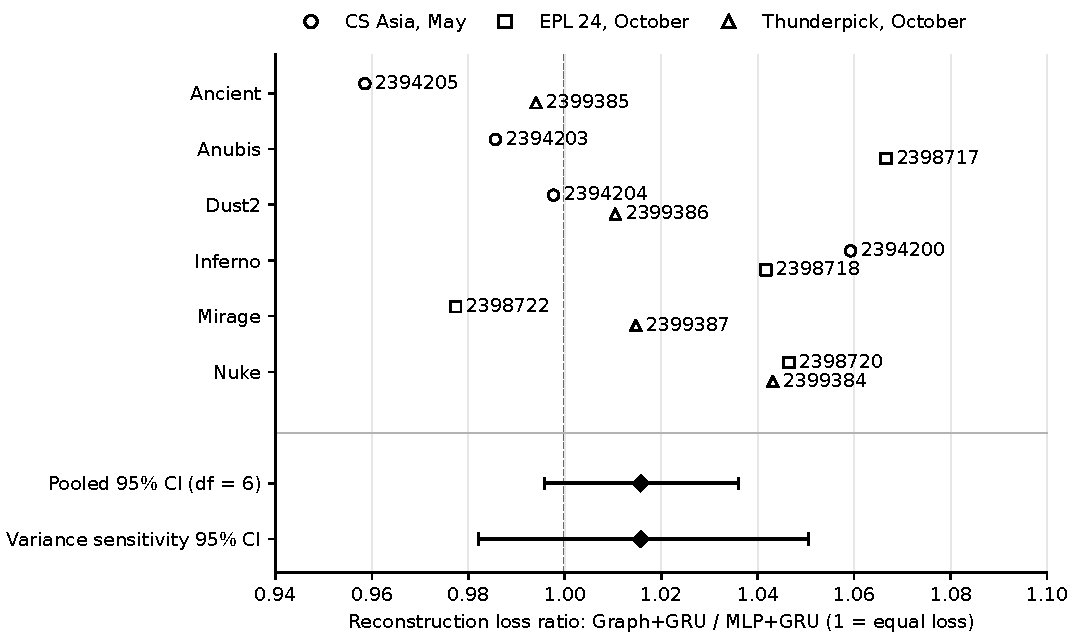
\includegraphics[width=\textwidth]{figures/independent_confirmation.pdf}
\caption{External technical confirmation. Open symbols show all 12 series, with shapes identifying the three events. Each series averages the three source-checkpoint seeds and its eligible windows. Diamonds and bars show the exponentiated equal-map mean log ratio and two prespecified, model-dependent 95\% intervals. They do not remove shared-team/event dependence. The source data table records every series and all six conditions.}
\label{fig:independent}
\end{figure*}

\begin{table}[t]
\caption{New-series reconstruction for the four core conditions. Losses average seeds and windows within series, then weight the six two-series map groups equally. Lower is better. Secondary conditions are descriptive.}
\label{tab:external}
\centering
\begin{tabular}{lr}
\toprule
Condition & Mean loss\\
\midrule
MLP static & 0.128612 \\ % [claim:C174] [evidence:E131]
MLP + GRU & 0.122492 \\ % [claim:C175] [evidence:E131]
Graph static & 0.129249 \\ % [claim:C176] [evidence:E131]
Graph + GRU & 0.124658 \\ % [claim:C177] [evidence:E131]
\bottomrule
\end{tabular}
\end{table}

The new-series state-only source prototypes accept 93.2\% of Graph+GRU query-seed assignments and 87.0\% for MLP+GRU. Their eligible seed-pair ARI means are 0.430 and 0.527, each from eighteen comparisons. Coverage is not calibrated confidence, and the method-specific common-accepted populations limit direct stability comparisons. % [claim:C190] [evidence:E134]

The recorded context is complete for 245 of the 246 new windows. One Inferno window retains unresolved HE release semantics; its affected counts remain unknown instead of being filled with zero. CT equipment and public score are available for all windows. The amendment and event-stage checks are detailed in Supplementary Appendix~D. % [claim:C191] [evidence:E150,E151]

For Graph+GRU plus joint context, acceptance is 91.3\% across all query-seed assignments and 91.7\% among the context-known subset. Seed ARI is 0.963 across eighteen eligible pairs, while agreement with context-only assignments is 1.000 on eighteen common-accepted comparisons. The source prototypes were already resource-dominated; neither conditional stability nor this agreement establishes tactical correctness. Availability and acceptance subsets differ from the state-only summaries. % [claim:C192] [evidence:E124,E152]

The complete seven-policy context intervention and weight-sensitivity table is in Supplementary Appendix~A-A. These controls change the observation weighting, rather than providing additional independent trials.

The telemetry correction follows the initial secondary analysis and is reported as an amendment; both result versions are retained. No source cluster, radius, context weight or encoder is refitted for these transfers. G4 has no same-map source candidates, so same-map retrieval is unsupported and all-source and other-map strata coincide. The evidence supports reporting computational transfer and telemetry limits; independent semantic retrieval validity remains unresolved.

The separate next-state prediction probe is retained in Supplementary Appendix~B-B; it is not the main representation endpoint.

\section{Discussion and Limitations}
\subsection{From a transferable representation to a tactical interpretation}
The shared input allows the same reconstruction and retrieval procedure to operate across the six maps. Its geometry and sampled motion describe recorded aspects of a defense; tactical interpretation also depends on information that these observations leave unresolved.

The new-series reconstruction estimate is consistent with the development warning against assuming a graph advantage. Temporal controls remain informative, while additional motion channels do not automatically improve this objective. In a separate development analysis, the highly stable joint clusters largely follow resources. These results motivate retaining deployment observations, contextual facets, and tactical judgments as separate evidence layers; no fixed place-to-duty rule follows from the current experiments. % [claim:C181] [evidence:E110,E124,E131]

\subsection{Implications for cross-map opening analysis}
The common representation makes it possible to pose the same reconstruction and comparison task across maps. The new-series experiment then tests a fixed model under target-map exclusion. Neither step supplies tactical labels. The difference matters when using the representation: a nearby source opening is evidence to inspect, and a stable cluster is a repeatable grouping in the selected observation space.

The resource diagnosis explains why context should remain visible to the analyst. If equipment accounts for most centroid separation, a cluster may summarize buying conditions more than a distinctive defensive arrangement. The appropriate follow-up is to inspect the associated deployment and its context together, rather than attach the same tactical duty to every occurrence of a map location. The limited pilot judgments do not yet show that new cross-map returns are useful for coaching.

\subsection{Selection, capacity and observation limitations}
The cohort is conditional on complete supplied windows and native observations. Excluding an early-ending window changes the population from arbitrary rounds to eligible openings; repeated windows and seeds do not compensate for the small number of series. The event-balanced sample is constrained by available metadata and archives, and two series per map provide little information about within-map residual distributions.

The graph and nongraph models share targets and a bottleneck, but their parameter counts and inductive biases differ. The comparison does not isolate topology as a causal factor, and permutation-averaging costs differ between the families. A low reconstruction loss can retain common resources or geography without preserving rare tactical distinctions. Endpoint motion, Euclidean geometry and global team observations also leave first-person visibility, intervening paths, opponent information and intent unresolved.

The context diagnosis concerns explicit weighting of an overlapping information branch. It does not demonstrate a resource-free latent space or select an optimal tactical weight. Missing telemetry, source-radius rejection and conditional ARI are separate filters; their retained populations should not be merged into a single accuracy or generalized to all openings.

\subsection{Scope of the project}
This CT study targets offline deployment representation and evidence retrieval. T-side openings, a production backend, coaching interventions, and win-rate effects are separate projects and have not been validated by the present experiments.

\section{Conclusion}
This study extends single-map defensive-opening analysis to a shared multi-map representation and a fixed transfer evaluation. Matched reconstruction controls make the roles of graph structure and learned temporal aggregation explicit. On new series, the recurrent graph model does not establish an advantage over its nongraph control. Context produces highly repeatable groups, but equipment can dominate their separation. These results support analyzing the recorded deployment and its context together, while preserving the distinction between a transferable representation and a validated tactical category. Independent retrieval relevance and coaching efficacy remain open. % [claim:C182] [evidence:E124,E126,E131]

\FloatBarrier
\bibliographystyle{IEEEtran}
\bibliography{references}
\end{document}
